\documentclass[10pt]{article}
\usepackage[a4paper,margin=18mm]{geometry}
\usepackage{amsmath,amssymb,booktabs,array,enumitem}
\usepackage[T1]{fontenc}\usepackage{lmodern}
\usepackage{tikz}\usetikzlibrary{shapes.gates.logic.US,positioning,arrows.meta,calc}
\usepackage[hidelinks]{hyperref}
\setlength{\parindent}{0pt}\setlength{\parskip}{4pt}\setlength{\emergencystretch}{2em}
\newcommand{\VDD}{V_{DD}}
\newcommand{\mos}[4]{\begin{scope}[shift={(#1,#2)}]
\draw(0,.23)--(0,-.23);\draw(0,.2)--(.25,.2)--(.25,.5);\draw(0,-.2)--(.25,-.2)--(.25,-.5);
\draw(-.16,.23)--(-.16,-.23);
\ifnum#4=1\draw(-.26,0)circle(.06);\draw(-.7,0)--(-.32,0);\else\draw(-.7,0)--(-.16,0);\fi
\node[anchor=east,font=\scriptsize]at(-.71,0){$#3$};\end{scope}}
\newcommand{\grd}[2]{\draw(#1,#2)--(#1,#2-.12);\draw(#1-.15,#2-.12)--(#1+.15,#2-.12);\draw(#1-.1,#2-.19)--(#1+.1,#2-.19);}
\newcommand{\rail}[3]{\draw(#1,#2)--(#1,#2+.2)node[above]{$#3$};}
\begin{document}\begin{center}{\Large\bfseries 2009 Midterm -- Corrected Solutions}\end{center}
\textbf{Scope.} All six Fall 2009 questions, 105 printed points. The three photographs contain incidental study notes; these are fallible comparisons, not a separate graded answer key. No process simulation is asserted.
\textbf{1. Brief answers}
\begin{enumerate}[label=(\alph*),leftmargin=7mm]
\item Design rules enforce manufacturable dimensions, spacing and enclosure/alignment tolerances for the actual process; they improve yield and electrical reliability.
\item NMOS implements $x_1\parallel(x_2x_3)\parallel x_4$; PMOS is its series/parallel dual $x_1(x_2\parallel x_3)x_4$. Every gate below has the true primary input, and the output is the required full complement.
\item Plasma processing can accumulate charge on a long conducting region attached to a gate. The gate oxide can then see a damaging voltage. Antenna rules limit that exposure; a protective diode or routing jump can discharge or avoid it.
\item Complementary pullup/pulldown networks give a full-rail stable Boolean output; ideally exactly one network conducts in a stable state; insulated gates give high input impedance; static state retention needs no periodic precharge clock. Leakage and finite switching current remain physical limitations. ``Every function is inverting'' and ``always exactly twice the number of inputs'' are not general properties.
\item A substrate ring tied to $V_{SS}$ and a well ring tied to $V_{DD}$ collect injected carriers and reduce the base-voltage excursions of the parasitic SCR pair.
\item Increase separation or shorten parallel overlap; insert a well-grounded shield (or route on suitable separated layers) and maintain a strong victim drive. A floating shield is not the same remedy.
\item An output rise draws $C_LV_{DD}^2$: half is stored and half dissipated in charging. The fall dissipates the stored half. One complete rise/fall cycle draws $C_LV_{DD}^2$, plus short-circuit and leakage energy.
\item Fanout gate capacitance, driver drain/diffusion capacitance, and interconnect capacitance (including coupling). Individual gate-oxide overlap/channel terms are subcomponents, not those three output-load categories.
\end{enumerate}
\begin{center}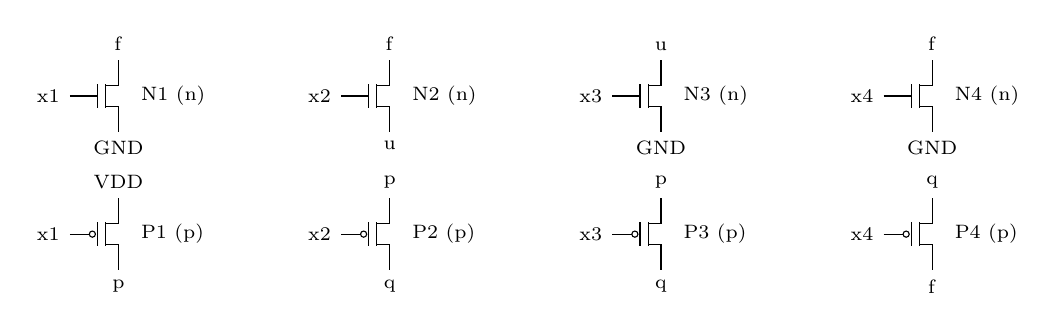
\begin{tikzpicture}[x=.65cm,y=.65cm,font=\scriptsize]
\mos{0.0}{0.0}{\mathrm{x1}}{0}
\draw(0.25,0.5)--(0.25,0.7)node[above]{$\mathrm{f}$};
\draw(0.25,-0.5)--(0.25,-0.7)node[below]{$\mathrm{GND}$};
\node[right]at(0.5,0.0){N1 (n)};
\mos{5.3}{0.0}{\mathrm{x2}}{0}
\draw(5.55,0.5)--(5.55,0.7)node[above]{$\mathrm{f}$};
\draw(5.55,-0.5)--(5.55,-0.7)node[below]{$\mathrm{u}$};
\node[right]at(5.8,0.0){N2 (n)};
\mos{10.6}{0.0}{\mathrm{x3}}{0}
\draw(10.85,0.5)--(10.85,0.7)node[above]{$\mathrm{u}$};
\draw(10.85,-0.5)--(10.85,-0.7)node[below]{$\mathrm{GND}$};
\node[right]at(11.1,0.0){N3 (n)};
\mos{15.899999999999999}{0.0}{\mathrm{x4}}{0}
\draw(16.15,0.5)--(16.15,0.7)node[above]{$\mathrm{f}$};
\draw(16.15,-0.5)--(16.15,-0.7)node[below]{$\mathrm{GND}$};
\node[right]at(16.4,0.0){N4 (n)};
\mos{0.0}{-2.7}{\mathrm{x1}}{1}
\draw(0.25,-2.2)--(0.25,-2.0)node[above]{$\mathrm{VDD}$};
\draw(0.25,-3.2)--(0.25,-3.4000000000000004)node[below]{$\mathrm{p}$};
\node[right]at(0.5,-2.7){P1 (p)};
\mos{5.3}{-2.7}{\mathrm{x2}}{1}
\draw(5.55,-2.2)--(5.55,-2.0)node[above]{$\mathrm{p}$};
\draw(5.55,-3.2)--(5.55,-3.4000000000000004)node[below]{$\mathrm{q}$};
\node[right]at(5.8,-2.7){P2 (p)};
\mos{10.6}{-2.7}{\mathrm{x3}}{1}
\draw(10.85,-2.2)--(10.85,-2.0)node[above]{$\mathrm{p}$};
\draw(10.85,-3.2)--(10.85,-3.4000000000000004)node[below]{$\mathrm{q}$};
\node[right]at(11.1,-2.7){P3 (p)};
\mos{15.899999999999999}{-2.7}{\mathrm{x4}}{1}
\draw(16.15,-2.2)--(16.15,-2.0)node[above]{$\mathrm{q}$};
\draw(16.15,-3.2)--(16.15,-3.4000000000000004)node[below]{$\mathrm{f}$};
\node[right]at(16.4,-2.7){P4 (p)};\end{tikzpicture}\\\small Eight physical MOS; all 16 input words checked. Equal terminal names denote connected wires. Bodies: nMOS to GND, pMOS to VDD.\end{center}
\newpage\textbf{2. Latchup circuit model}
\begin{center}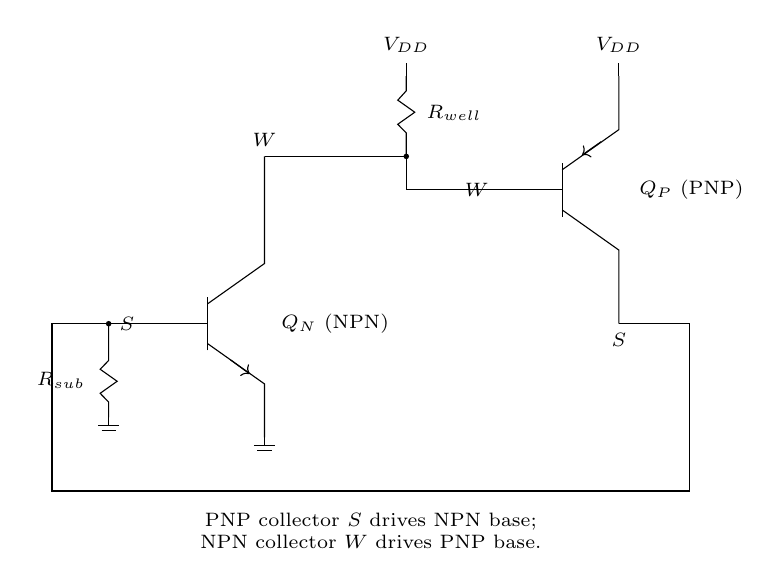
\begin{tikzpicture}[x=.9cm,y=.85cm,font=\scriptsize]
\draw(1.7,1.6)--(1.7,2.4);\draw(1.7,2.3)--(2.5,2.9)--(2.5,4.5);\draw(1.7,1.7)--(2.5,1.1)--(2.5,.3);\draw[->](2.02,1.46)--(2.29,1.25);\draw(.8,2)--(1.7,2);\node[right]at(2.6,2){$Q_N$ (NPN)};\node[left]at(.8,2){$S$};\node[above]at(2.5,4.5){$W$};\grd{2.5}{.3}
\draw(6.7,3.6)--(6.7,4.4);\draw(6.7,4.3)--(7.5,4.9)--(7.5,5.7);\draw[->](7.25,4.72)--(6.98,4.52);\draw(6.7,3.7)--(7.5,3.1)--(7.5,2);\draw(5.8,4)--(6.7,4);\node[right]at(7.65,4){$Q_P$ (PNP)};\rail{7.5}{5.7}{V_{DD}}\node[left]at(5.8,4){$W$};\node[below]at(7.5,2){$S$};
\draw(2.5,4.5)--(4.5,4.5)--(4.5,4)--(5.8,4);\draw(.8,2)--(-.5,2)--(-.5,-.5)--(8.5,-.5)--(8.5,2)--(7.5,2);
\draw(4.5,4.5)--(4.5,4.85)--(4.38,4.98)--(4.62,5.16)--(4.38,5.34)--(4.5,5.48)--(4.5,5.7);\rail{4.5}{5.7}{V_{DD}}\node[right]at(4.65,5.15){$R_{well}$};\draw(.3,2)--(.3,1.45)--(.18,1.32)--(.42,1.14)--(.18,.96)--(.3,.83)--(.3,.6);\grd{.3}{.6}\node[left]at(.1,1.15){$R_{sub}$};\fill(.3,2)circle(1pt);\fill(4.5,4.5)circle(1pt);\node[align=center]at(4,-1.1){PNP collector $S$ drives NPN base;\\NPN collector $W$ drives PNP base.};\end{tikzpicture}\end{center}

The circuit connects PNP collector S to the NPN base and NPN collector W to the PNP base, with both base shunts shown. Current injected into substrate node S raises the NPN base. Its collector current through $R_{well}$ lowers well node W and turns on the PNP; PNP collector current reinforces S. The regenerative loop can latch a low-impedance $V_{DD}$--$V_{SS}$ path if the loop gain is sufficient (the ideal SCR criterion can be written $\alpha_{PNP}+\alpha_{NPN}\ge1$). It persists until the current drops below its holding condition. Guard rings/taps reduce the shunt resistances and collect carriers; they suppress triggering rather than inserting a resistor in the intended logic channel.
\newpage\textbf{3. Short-circuit power in the literal chains}
\begin{center}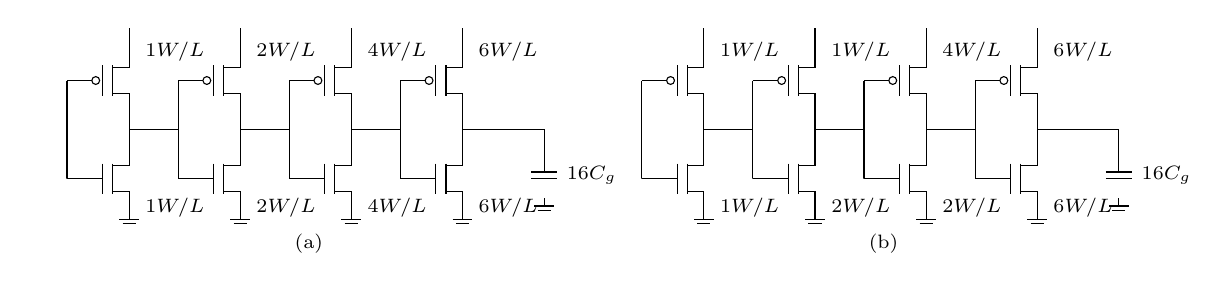
\begin{tikzpicture}[x=.83cm,y=.83cm,font=\scriptsize]\begin{scope}[xshift=0cm]
\mos{0.0}{2.5}{\phantom{X}}{1}\mos{0.0}{1}{\phantom{X}}{0}
\draw(0.25,3)--(0.25,3.3);\draw(0.25,2)--(0.25,1.5);\grd{0.25}{.5}
\draw(-0.7,2.5)--(-0.7,1)--(-0.7,1.75);
\node[above right]at(0.35,2.65){$1W/L$};\node[below right]at(0.35,.85){$1W/L$};
\draw(0.25,1.75)--(1.0,1.75);
\mos{1.7}{2.5}{\phantom{X}}{1}\mos{1.7}{1}{\phantom{X}}{0}
\draw(1.95,3)--(1.95,3.3);\draw(1.95,2)--(1.95,1.5);\grd{1.95}{.5}
\draw(1.0,2.5)--(1.0,1)--(1.0,1.75);
\node[above right]at(2.05,2.65){$2W/L$};\node[below right]at(2.05,.85){$2W/L$};
\draw(1.95,1.75)--(2.7,1.75);
\mos{3.4}{2.5}{\phantom{X}}{1}\mos{3.4}{1}{\phantom{X}}{0}
\draw(3.65,3)--(3.65,3.3);\draw(3.65,2)--(3.65,1.5);\grd{3.65}{.5}
\draw(2.7,2.5)--(2.7,1)--(2.7,1.75);
\node[above right]at(3.75,2.65){$4W/L$};\node[below right]at(3.75,.85){$4W/L$};
\draw(3.65,1.75)--(4.4,1.75);
\mos{5.1}{2.5}{\phantom{X}}{1}\mos{5.1}{1}{\phantom{X}}{0}
\draw(5.35,3)--(5.35,3.3);\draw(5.35,2)--(5.35,1.5);\grd{5.35}{.5}
\draw(4.3999999999999995,2.5)--(4.3999999999999995,1)--(4.3999999999999995,1.75);
\node[above right]at(5.449999999999999,2.65){$6W/L$};\node[below right]at(5.449999999999999,.85){$6W/L$};
\draw(5.35,1.75)--(6.6,1.75)--(6.6,1.1);\draw(6.4,1.1)--(6.8,1.1) (6.4,1)--(6.8,1);\grd{6.6}{.7}\node[right]at(6.8,1.05){$16C_g$};
\node at(3,0){(a)};
\end{scope}\begin{scope}[xshift=7.3cm]
\mos{0.0}{2.5}{\phantom{X}}{1}\mos{0.0}{1}{\phantom{X}}{0}
\draw(0.25,3)--(0.25,3.3);\draw(0.25,2)--(0.25,1.5);\grd{0.25}{.5}
\draw(-0.7,2.5)--(-0.7,1)--(-0.7,1.75);
\node[above right]at(0.35,2.65){$1W/L$};\node[below right]at(0.35,.85){$1W/L$};
\draw(0.25,1.75)--(1.0,1.75);
\mos{1.7}{2.5}{\phantom{X}}{1}\mos{1.7}{1}{\phantom{X}}{0}
\draw(1.95,3)--(1.95,3.3);\draw(1.95,2)--(1.95,1.5);\grd{1.95}{.5}
\draw(1.0,2.5)--(1.0,1)--(1.0,1.75);
\node[above right]at(2.05,2.65){$1W/L$};\node[below right]at(2.05,.85){$2W/L$};
\draw(1.95,1.75)--(2.7,1.75);
\mos{3.4}{2.5}{\phantom{X}}{1}\mos{3.4}{1}{\phantom{X}}{0}
\draw(3.65,3)--(3.65,3.3);\draw(3.65,2)--(3.65,1.5);\grd{3.65}{.5}
\draw(2.7,2.5)--(2.7,1)--(2.7,1.75);
\node[above right]at(3.75,2.65){$4W/L$};\node[below right]at(3.75,.85){$2W/L$};
\draw(3.65,1.75)--(4.4,1.75);
\mos{5.1}{2.5}{\phantom{X}}{1}\mos{5.1}{1}{\phantom{X}}{0}
\draw(5.35,3)--(5.35,3.3);\draw(5.35,2)--(5.35,1.5);\grd{5.35}{.5}
\draw(4.3999999999999995,2.5)--(4.3999999999999995,1)--(4.3999999999999995,1.75);
\node[above right]at(5.449999999999999,2.65){$6W/L$};\node[below right]at(5.449999999999999,.85){$6W/L$};
\draw(5.35,1.75)--(6.6,1.75)--(6.6,1.1);\draw(6.4,1.1)--(6.8,1.1) (6.4,1)--(6.8,1);\grd{6.6}{.7}\node[right]at(6.8,1.05){$16C_g$};
\node at(3,0){(b)};
\end{scope}\end{tikzpicture}\end{center}

All widths in Figure 2 are read literally. Equal p/n widths are \emph{not} balanced here: $\mu_n=2\mu_p$, so $R_n=R/w_n$ and $R_p=2R/w_p$. With no drain/wire capacitance, the following transition-time estimates are in $RC_g$ units:
\begin{center}\begin{tabular}{ccccccc}\toprule Chain&Stage&$w_p$&$w_n$&$C_{out}/C_g$&$t_r/RC_g$&$t_f/RC_g$\\\midrule
(a)&1&1&1&4&8&4\\ &(2)&2&2&8&8&4\\ &(3)&4&4&12&6&3\\ &(4)&6&6&16&$16/3$&$8/3$\\\midrule
(b)&1&1&1&3&6&3\\ &(2)&1&2&6&12&3\\ &(3)&4&2&12&6&6\\ &(4)&6&6&16&$16/3$&$8/3$\\\bottomrule\end{tabular}\end{center}
\textbf{Classroom conclusion: (a) has slightly lower short-circuit power under a common square-law overlap approximation.} It is incorrect to identify short-circuit power just with the switched output capacitance. Chain (b) has less total switched capacitance ($37C_g$ versus $40C_g$), which answers a different power component.

Because the pairs are unbalanced, the equal-$\beta$ formula must be generalized. Let $\beta_n=\beta_0w_n$, $\beta_p=\beta_0w_p/2$, $\Delta=V_{DD}-V_{Tn}-|V_{Tp}|>0$, and
\[b(\beta_n,\beta_p)=\frac{\beta_n\beta_p}{(\sqrt{\beta_n}+\sqrt{\beta_p})^2}.\]
For a linear input ramp, the approximate overlap current is $\tfrac12\min\{\beta_n u^2,\beta_p(\Delta-u)^2\}$. Integrating the two branches on either side of $u=\sqrt{\beta_p}\Delta/(\sqrt{\beta_n}+\sqrt{\beta_p})$ yields
\[P_{sc}\simeq\frac{f\Delta^3}{6}\sum_i b_i(t_{r,in,i}+t_{f,in,i}).\]
This reduces to $\beta\tau\Delta^3f/12$ for a balanced inverter with $t_{r,in}=t_{f,in}=\tau$. First-stage contributions cancel because both chains have the same first pair and external input. Let $q=3-2\sqrt2$, so $b_{a,i}/\beta_0=q[1,2,4,6]$ and $b_{b,i}/\beta_0=[q,2/9,1/2,6q]$. The last three stages give
\begin{align*}
S_a/(\beta_0RC_g)&=2q(8+4)+4q(8+4)+6q(6+3)=126q,\\
S_b/(\beta_0RC_g)&=(2/9)(6+3)+(1/2)(12+3)+6q(6+6)=19/2+72q,\\
(S_b-S_a)/(\beta_0RC_g)&=19/2-54q\approx .235065>0.
\end{align*}
The advantage is small in this declared model.  \textbf{A universal physical ordering is not determined by $R,C_g,\mu_n/\mu_p$ alone}: the exam omits thresholds, waveform shape, frequency and a finite-load current model. Loading suppresses actual overlap current and changes output slews. The result above is an explicit analytical classroom estimate; it is not a claimed SPICE measurement. If $\Delta\le0$, this ideal overlap model predicts zero for both, rather than a strict ordering.

\newpage\textbf{4. Power, actual fanouts and conditional dual-threshold assignment}
\begin{center}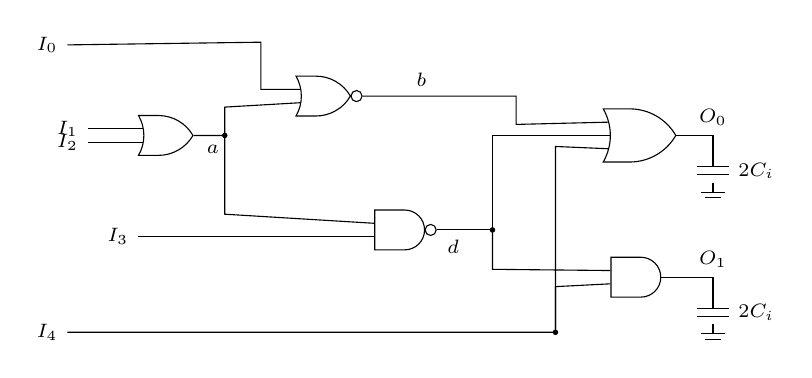
\begin{tikzpicture}[x=1cm,y=1cm,font=\scriptsize]
\node[or gate US,draw,logic gate inputs=nn](a)at(1,2){};
\node[nor gate US,draw,logic gate inputs=nn](b)at(3,2.5){};
\node[nand gate US,draw,logic gate inputs=nn](d)at(4,.8){};
\node[or gate US,draw,logic gate inputs=nnn](o0)at(7,2){};
\node[and gate US,draw,logic gate inputs=nn](o1)at(7,.2){};
\draw(a.input 1)--++(-.7,0)node[left]{$I_1$};\draw(a.input 2)--++(-.7,0)node[left]{$I_2$};
\draw(b.input 1)--++(-.5,0)--++(0,.6)--(-.2,3.15)node[left]{$I_0$};
\draw(a.output)--(1.8,2)coordinate(j)--(1.8,2.36)--(b.input 2);\fill(j)circle(1pt);\node[below]at(1.65,2){$a$};
\draw(j)--(1.8,1)--(d.input 1);\draw(d.input 2)--++(-3,0)node[left]{$I_3$};
\draw(b.output)--(5.5,2.5)--(5.5,2.14)--(o0.input 1);\node[above]at(4.3,2.5){$b$};
\draw(d.output)--(5.2,.8)coordinate(k)--(5.2,2)--(o0.input 2);\fill(k)circle(1pt);\node[below]at(4.7,.8){$d$};
\draw(k)--(5.2,.3)--(o1.input 1);\draw(-.2,-.5)node[left]{$I_4$}--(6,-.5)coordinate(l)--(6,.08)--(o1.input 2);
\draw(l)--(6,1.86)--(o0.input 3);\fill(l)circle(1pt);
\draw(o0.output)--(8,2)node[above]{$O_0$}--(8,1.6);\draw(7.8,1.6)--(8.2,1.6) (7.8,1.5)--(8.2,1.5);\grd{8}{1.4}\node[right]at(8.2,1.55){$2C_i$};
\draw(o1.output)--(8,.2)node[above]{$O_1$}--(8,-.2);\draw(7.8,-.2)--(8.2,-.2) (7.8,-.3)--(8.2,-.3);\grd{8}{-.4}\node[right]at(8.2,-.25){$2C_i$};
\end{tikzpicture}\end{center}
Let $a=I_1+I_2$, $b=\overline{I_0+a}$, $d=\overline{aI_3}$. Then $O_0=b+d+I_4$ and $O_1=dI_4$. The original first gate is a two-input OR, and the final upper gate is a three-input OR. Neither handwritten arcs nor conventional expectations add input/output bubbles.
\begin{center}\begin{tabular}{ccccc}\toprule $I_0I_1I_2I_3I_4$&a&b&d&$(O_0,O_1)$\\\midrule01001&1&0&1&(1,1)\\11011&1&0&0&(1,0)\\11100&1&0&1&(1,0)\\01101&1&0&1&(1,1)\\\bottomrule\end{tabular}\end{center}
(a) Under the intended fully settled, no-glitch capacitive model, the largest charge in one input interval is $2C_iV_{DD}^2$: d rises on the second transition, and $O_1$ rises on the third. With $f$ interpreted as input-interval rate,
\[\boxed{P_{peak,\,interval}=2fC_iV_{DD}^2.}\]
This is a maximum \emph{interval-averaged switching estimate}, not instantaneous $V_{DD}I(t)$, which needs transition/current data. Over the four-step repeating cycle, visible gate-output charging totals $4C_iV_{DD}^2$, giving average $fC_iV_{DD}^2$. A conventional AND2 is NAND2 plus inverter; its internal node also rises once, adding $C_iV_{DD}^2$ per cycle and raising that mean to $5fC_iV_{DD}^2/4$. It does not change the maximum settled interval above. First OR and final OR internal nodes remain constant for the settled words.

The source does not promise glitch-free transitions. In $11011\to11100$, $I_4$ falls directly while d rises after the NAND delay; the inputs of the final OR temporarily can all be zero. Its physical internal/output pulse depends on arc delays and inertial/transistor behavior. Therefore the steady-word table cannot establish actual peak or glitch power. Input slew, thresholds, leakage and a switching-time model would be needed. The written ``peak power'' is retained; no instantaneous numerical claim is fabricated.

(b) Assume the reference inverter is mobility-balanced, so its p/n ON resistances are the same $R_0$ and one unit is $R_0C_i$. Each physical gate input has $C_i$. OR/AND uses its ordinary complementary gate followed by an inverter, including that inverter's gate load. Worst rise/fall mean estimates give:
\begin{center}\begin{tabular}{ccccc}\toprule Gate&Implementation&External load&Internal load&Mean delay units\\\midrule
a&NOR2 + INV&$2C_i$&$C_i$&$1.5+2=3.5$\\
b&NOR2&$C_i$&--&$1.5$\\
d&NAND2&$2C_i$&--&$3$\\
$O_0$&NOR3 + INV&$2C_i$&$C_i$&$2+2=4$\\
$O_1$&NAND2 + INV&$2C_i$&$C_i$&$1.5+2=3.5$\\\bottomrule\end{tabular}\end{center}
Ignoring the actual two-gate fanout changes the answer. If mobility balance is not a class convention, let $r_p+r_n=2$ in reference units. Then the five means are $(2r_p+r_n)/2+2$, $(2r_p+r_n)/2$, $r_p+2r_n$, $(3r_p+r_n)/2+2$, and $(r_p+2r_n)/2+2$. The stated dimensions alone do not provide mobility.

(c) The conservative original physical paths are $a\to d\to O_0=10.5$, $a\to b\to O_0=9$, and $a\to d\to O_1=10$ units. One conditional allocation puts b's four NOR2 devices at high $V_T$ and retains all other devices at low $V_T$, provided its added delay is at most 1.5 units. The source's threshold-symbol convention is reproduced below (device type is also stated explicitly):
\begin{center}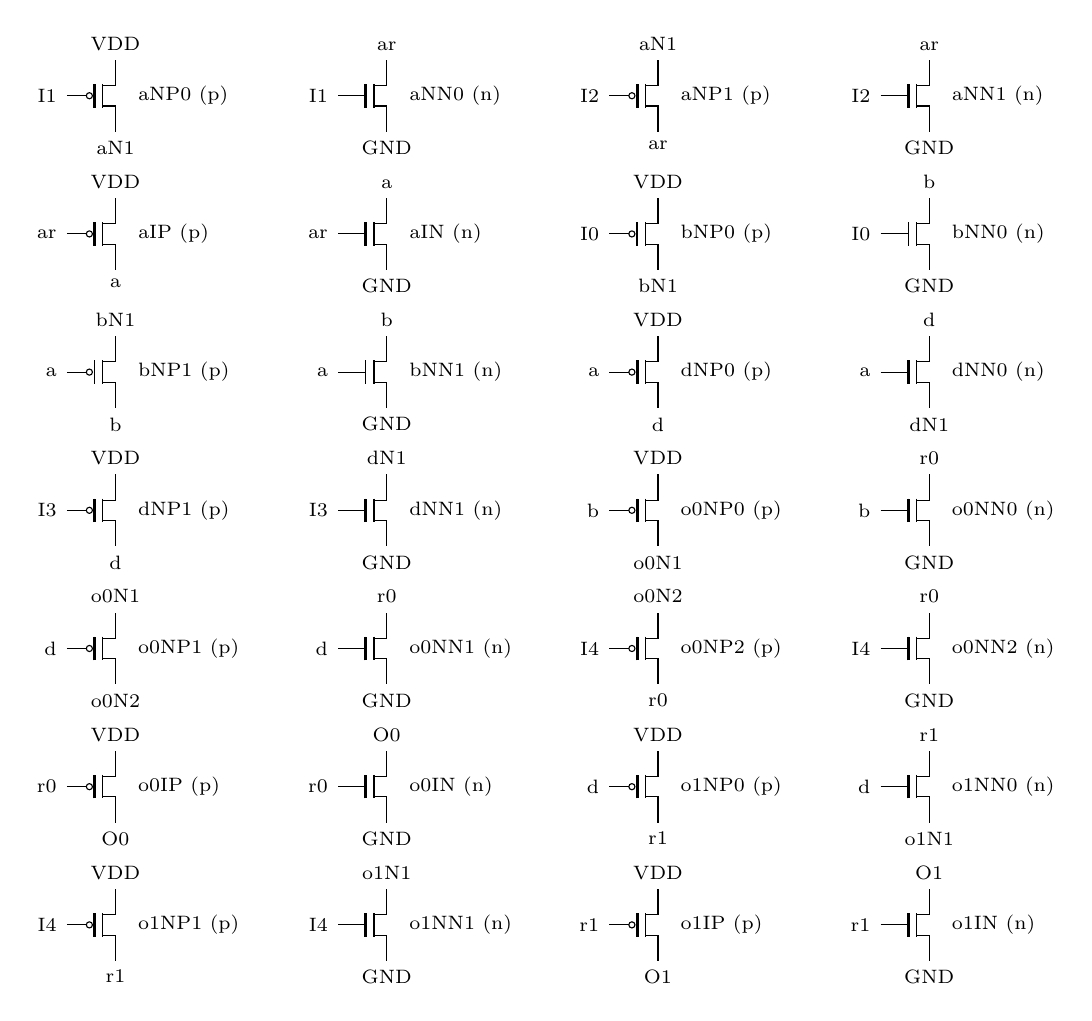
\begin{tikzpicture}[x=.65cm,y=.65cm,font=\scriptsize]
\mos{0.0}{0.0}{\mathrm{I1}}{1}
\draw(0.25,0.5)--(0.25,0.7)node[above]{$\mathrm{VDD}$};
\draw(0.25,-0.5)--(0.25,-0.7)node[below]{$\mathrm{aN1}$};
\node[right]at(0.5,0.0){aNP0 (p)};
\draw[line width=1.1pt](-0.16,-0.23)--(-0.16,0.23);
\mos{5.3}{0.0}{\mathrm{I1}}{0}
\draw(5.55,0.5)--(5.55,0.7)node[above]{$\mathrm{ar}$};
\draw(5.55,-0.5)--(5.55,-0.7)node[below]{$\mathrm{GND}$};
\node[right]at(5.8,0.0){aNN0 (n)};
\draw[line width=1.1pt](5.14,-0.23)--(5.14,0.23);
\mos{10.6}{0.0}{\mathrm{I2}}{1}
\draw(10.85,0.5)--(10.85,0.7)node[above]{$\mathrm{aN1}$};
\draw(10.85,-0.5)--(10.85,-0.7)node[below]{$\mathrm{ar}$};
\node[right]at(11.1,0.0){aNP1 (p)};
\draw[line width=1.1pt](10.44,-0.23)--(10.44,0.23);
\mos{15.899999999999999}{0.0}{\mathrm{I2}}{0}
\draw(16.15,0.5)--(16.15,0.7)node[above]{$\mathrm{ar}$};
\draw(16.15,-0.5)--(16.15,-0.7)node[below]{$\mathrm{GND}$};
\node[right]at(16.4,0.0){aNN1 (n)};
\draw[line width=1.1pt](15.739999999999998,-0.23)--(15.739999999999998,0.23);
\mos{0.0}{-2.7}{\mathrm{ar}}{1}
\draw(0.25,-2.2)--(0.25,-2.0)node[above]{$\mathrm{VDD}$};
\draw(0.25,-3.2)--(0.25,-3.4000000000000004)node[below]{$\mathrm{a}$};
\node[right]at(0.5,-2.7){aIP (p)};
\draw[line width=1.1pt](-0.16,-2.93)--(-0.16,-2.47);
\mos{5.3}{-2.7}{\mathrm{ar}}{0}
\draw(5.55,-2.2)--(5.55,-2.0)node[above]{$\mathrm{a}$};
\draw(5.55,-3.2)--(5.55,-3.4000000000000004)node[below]{$\mathrm{GND}$};
\node[right]at(5.8,-2.7){aIN (n)};
\draw[line width=1.1pt](5.14,-2.93)--(5.14,-2.47);
\mos{10.6}{-2.7}{\mathrm{I0}}{1}
\draw(10.85,-2.2)--(10.85,-2.0)node[above]{$\mathrm{VDD}$};
\draw(10.85,-3.2)--(10.85,-3.4000000000000004)node[below]{$\mathrm{bN1}$};
\node[right]at(11.1,-2.7){bNP0 (p)};
\mos{15.899999999999999}{-2.7}{\mathrm{I0}}{0}
\draw(16.15,-2.2)--(16.15,-2.0)node[above]{$\mathrm{b}$};
\draw(16.15,-3.2)--(16.15,-3.4000000000000004)node[below]{$\mathrm{GND}$};
\node[right]at(16.4,-2.7){bNN0 (n)};
\mos{0.0}{-5.4}{\mathrm{a}}{1}
\draw(0.25,-4.9)--(0.25,-4.7)node[above]{$\mathrm{bN1}$};
\draw(0.25,-5.9)--(0.25,-6.1000000000000005)node[below]{$\mathrm{b}$};
\node[right]at(0.5,-5.4){bNP1 (p)};
\mos{5.3}{-5.4}{\mathrm{a}}{0}
\draw(5.55,-4.9)--(5.55,-4.7)node[above]{$\mathrm{b}$};
\draw(5.55,-5.9)--(5.55,-6.1000000000000005)node[below]{$\mathrm{GND}$};
\node[right]at(5.8,-5.4){bNN1 (n)};
\mos{10.6}{-5.4}{\mathrm{a}}{1}
\draw(10.85,-4.9)--(10.85,-4.7)node[above]{$\mathrm{VDD}$};
\draw(10.85,-5.9)--(10.85,-6.1000000000000005)node[below]{$\mathrm{d}$};
\node[right]at(11.1,-5.4){dNP0 (p)};
\draw[line width=1.1pt](10.44,-5.630000000000001)--(10.44,-5.17);
\mos{15.899999999999999}{-5.4}{\mathrm{a}}{0}
\draw(16.15,-4.9)--(16.15,-4.7)node[above]{$\mathrm{d}$};
\draw(16.15,-5.9)--(16.15,-6.1000000000000005)node[below]{$\mathrm{dN1}$};
\node[right]at(16.4,-5.4){dNN0 (n)};
\draw[line width=1.1pt](15.739999999999998,-5.630000000000001)--(15.739999999999998,-5.17);
\mos{0.0}{-8.100000000000001}{\mathrm{I3}}{1}
\draw(0.25,-7.600000000000001)--(0.25,-7.400000000000001)node[above]{$\mathrm{VDD}$};
\draw(0.25,-8.600000000000001)--(0.25,-8.8)node[below]{$\mathrm{d}$};
\node[right]at(0.5,-8.100000000000001){dNP1 (p)};
\draw[line width=1.1pt](-0.16,-8.330000000000002)--(-0.16,-7.870000000000001);
\mos{5.3}{-8.100000000000001}{\mathrm{I3}}{0}
\draw(5.55,-7.600000000000001)--(5.55,-7.400000000000001)node[above]{$\mathrm{dN1}$};
\draw(5.55,-8.600000000000001)--(5.55,-8.8)node[below]{$\mathrm{GND}$};
\node[right]at(5.8,-8.100000000000001){dNN1 (n)};
\draw[line width=1.1pt](5.14,-8.330000000000002)--(5.14,-7.870000000000001);
\mos{10.6}{-8.100000000000001}{\mathrm{b}}{1}
\draw(10.85,-7.600000000000001)--(10.85,-7.400000000000001)node[above]{$\mathrm{VDD}$};
\draw(10.85,-8.600000000000001)--(10.85,-8.8)node[below]{$\mathrm{o0N1}$};
\node[right]at(11.1,-8.100000000000001){o0NP0 (p)};
\draw[line width=1.1pt](10.44,-8.330000000000002)--(10.44,-7.870000000000001);
\mos{15.899999999999999}{-8.100000000000001}{\mathrm{b}}{0}
\draw(16.15,-7.600000000000001)--(16.15,-7.400000000000001)node[above]{$\mathrm{r0}$};
\draw(16.15,-8.600000000000001)--(16.15,-8.8)node[below]{$\mathrm{GND}$};
\node[right]at(16.4,-8.100000000000001){o0NN0 (n)};
\draw[line width=1.1pt](15.739999999999998,-8.330000000000002)--(15.739999999999998,-7.870000000000001);
\mos{0.0}{-10.8}{\mathrm{d}}{1}
\draw(0.25,-10.3)--(0.25,-10.100000000000001)node[above]{$\mathrm{o0N1}$};
\draw(0.25,-11.3)--(0.25,-11.5)node[below]{$\mathrm{o0N2}$};
\node[right]at(0.5,-10.8){o0NP1 (p)};
\draw[line width=1.1pt](-0.16,-11.030000000000001)--(-0.16,-10.57);
\mos{5.3}{-10.8}{\mathrm{d}}{0}
\draw(5.55,-10.3)--(5.55,-10.100000000000001)node[above]{$\mathrm{r0}$};
\draw(5.55,-11.3)--(5.55,-11.5)node[below]{$\mathrm{GND}$};
\node[right]at(5.8,-10.8){o0NN1 (n)};
\draw[line width=1.1pt](5.14,-11.030000000000001)--(5.14,-10.57);
\mos{10.6}{-10.8}{\mathrm{I4}}{1}
\draw(10.85,-10.3)--(10.85,-10.100000000000001)node[above]{$\mathrm{o0N2}$};
\draw(10.85,-11.3)--(10.85,-11.5)node[below]{$\mathrm{r0}$};
\node[right]at(11.1,-10.8){o0NP2 (p)};
\draw[line width=1.1pt](10.44,-11.030000000000001)--(10.44,-10.57);
\mos{15.899999999999999}{-10.8}{\mathrm{I4}}{0}
\draw(16.15,-10.3)--(16.15,-10.100000000000001)node[above]{$\mathrm{r0}$};
\draw(16.15,-11.3)--(16.15,-11.5)node[below]{$\mathrm{GND}$};
\node[right]at(16.4,-10.8){o0NN2 (n)};
\draw[line width=1.1pt](15.739999999999998,-11.030000000000001)--(15.739999999999998,-10.57);
\mos{0.0}{-13.5}{\mathrm{r0}}{1}
\draw(0.25,-13.0)--(0.25,-12.8)node[above]{$\mathrm{VDD}$};
\draw(0.25,-14.0)--(0.25,-14.2)node[below]{$\mathrm{O0}$};
\node[right]at(0.5,-13.5){o0IP (p)};
\draw[line width=1.1pt](-0.16,-13.73)--(-0.16,-13.27);
\mos{5.3}{-13.5}{\mathrm{r0}}{0}
\draw(5.55,-13.0)--(5.55,-12.8)node[above]{$\mathrm{O0}$};
\draw(5.55,-14.0)--(5.55,-14.2)node[below]{$\mathrm{GND}$};
\node[right]at(5.8,-13.5){o0IN (n)};
\draw[line width=1.1pt](5.14,-13.73)--(5.14,-13.27);
\mos{10.6}{-13.5}{\mathrm{d}}{1}
\draw(10.85,-13.0)--(10.85,-12.8)node[above]{$\mathrm{VDD}$};
\draw(10.85,-14.0)--(10.85,-14.2)node[below]{$\mathrm{r1}$};
\node[right]at(11.1,-13.5){o1NP0 (p)};
\draw[line width=1.1pt](10.44,-13.73)--(10.44,-13.27);
\mos{15.899999999999999}{-13.5}{\mathrm{d}}{0}
\draw(16.15,-13.0)--(16.15,-12.8)node[above]{$\mathrm{r1}$};
\draw(16.15,-14.0)--(16.15,-14.2)node[below]{$\mathrm{o1N1}$};
\node[right]at(16.4,-13.5){o1NN0 (n)};
\draw[line width=1.1pt](15.739999999999998,-13.73)--(15.739999999999998,-13.27);
\mos{0.0}{-16.200000000000003}{\mathrm{I4}}{1}
\draw(0.25,-15.700000000000003)--(0.25,-15.500000000000004)node[above]{$\mathrm{VDD}$};
\draw(0.25,-16.700000000000003)--(0.25,-16.900000000000002)node[below]{$\mathrm{r1}$};
\node[right]at(0.5,-16.200000000000003){o1NP1 (p)};
\draw[line width=1.1pt](-0.16,-16.430000000000003)--(-0.16,-15.970000000000002);
\mos{5.3}{-16.200000000000003}{\mathrm{I4}}{0}
\draw(5.55,-15.700000000000003)--(5.55,-15.500000000000004)node[above]{$\mathrm{o1N1}$};
\draw(5.55,-16.700000000000003)--(5.55,-16.900000000000002)node[below]{$\mathrm{GND}$};
\node[right]at(5.8,-16.200000000000003){o1NN1 (n)};
\draw[line width=1.1pt](5.14,-16.430000000000003)--(5.14,-15.970000000000002);
\mos{10.6}{-16.200000000000003}{\mathrm{r1}}{1}
\draw(10.85,-15.700000000000003)--(10.85,-15.500000000000004)node[above]{$\mathrm{VDD}$};
\draw(10.85,-16.700000000000003)--(10.85,-16.900000000000002)node[below]{$\mathrm{O1}$};
\node[right]at(11.1,-16.200000000000003){o1IP (p)};
\draw[line width=1.1pt](10.44,-16.430000000000003)--(10.44,-15.970000000000002);
\mos{15.899999999999999}{-16.200000000000003}{\mathrm{r1}}{0}
\draw(16.15,-15.700000000000003)--(16.15,-15.500000000000004)node[above]{$\mathrm{O1}$};
\draw(16.15,-16.700000000000003)--(16.15,-16.900000000000002)node[below]{$\mathrm{GND}$};
\node[right]at(16.4,-16.200000000000003){o1IN (n)};
\draw[line width=1.1pt](15.739999999999998,-16.430000000000003)--(15.739999999999998,-15.970000000000002);\end{tikzpicture}\\\small 28 physical MOS. Only bN devices are high-VT in this conditional example. Equal terminal names denote connected wires. Bodies: nMOS to GND, pMOS to VDD.\end{center}
If the added delay of the final AND is at most .5 units, its six devices can also be high-$V_T$ under that conservative timing envelope. These are feasible examples, not a proven unique leakage optimum. The question supplies no high-$V_T$ penalty, leakage currents or polarity-specific arc model, so an unconditional minimum-leakage transistor assignment cannot be derived. Within the four settled words $O_0$ is constant, but deleting its physical paths would be a separate logic optimization and would miss the possible hazard above.
\newpage\textbf{5. TSV manufacturing order}
\begin{center}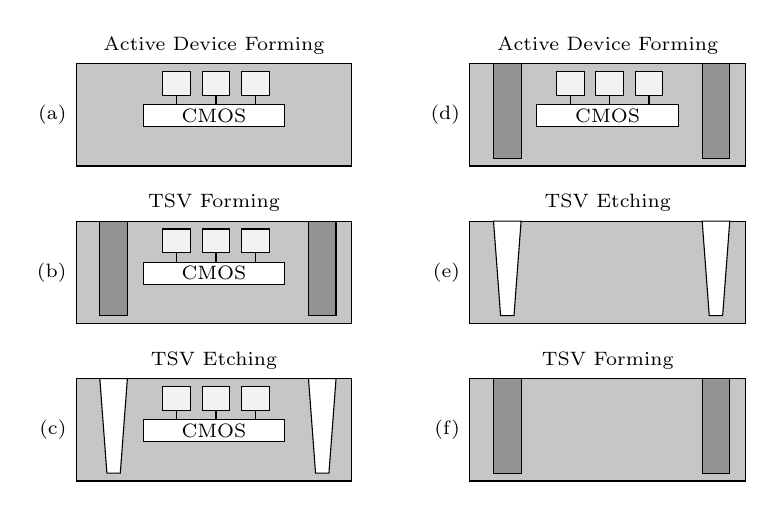
\begin{tikzpicture}[x=1cm,y=1cm,font=\scriptsize]
\foreach\x/\y/\a/\title/\active/\hole/\fillvia in{0/4/a/Active Device Forming/1/0/0,5/4/d/Active Device Forming/1/0/1,0/2/b/TSV Forming/1/0/1,5/2/e/TSV Etching/0/1/0,0/0/c/TSV Etching/1/1/0,5/0/f/TSV Forming/0/0/1}{
\begin{scope}[shift={(\x,\y)}]\draw[fill=gray!45](0,0)rectangle(3.5,1.3);\node[above]at(1.75,1.3){\title};\node[left]at(0,.65){(\a)};
\ifnum\active=1\draw[fill=white](.85,.5)rectangle(2.65,.78);\node at(1.75,.64){CMOS};\foreach\t in{1.1,1.6,2.1}{\draw[fill=gray!10](\t,.9)rectangle(\t+.35,1.2);\draw(\t+.175,.78)--(\t+.175,.9);}\fi
\ifnum\hole=1\foreach\t in{.3,2.95}{\draw[fill=white](\t,1.3)--(\t+.35,1.3)--(\t+.26,.1)--(\t+.09,.1)--cycle;}\fi
\ifnum\fillvia=1\foreach\t in{.3,2.95}{\draw[fill=gray!85](\t,.1)rectangle(\t+.35,1.3);}\fi
\end{scope}}
\end{tikzpicture}\\Figure 4: Partial manufacturing steps; schematic cross sections normalized.\end{center}
Via-first: \boxed{(e)\to(f)\to(d)}. Etch the bare substrate, form/fill the TSV, then form active devices in the substrate already containing TSVs.

Via-last: \boxed{(a)\to(c)\to(b)}. Form active devices, etch vias in that processed substrate, then form/fill them. The two ``Active Device Forming'' panels differ in whether their vias already exist. Naming conventions can include via-middle in other flows; these six source panels fix this exercise's ordering. See the primary \href{https://pubs.aip.org/avs/jva/article/38/3/031202/1023659/Tutorial-on-forming-through-silicon-vias}{TSV process tutorial} for the distinction relative to FEOL/BEOL.
\newpage\textbf{6. Boolean function and reachable RC networks}
\begin{center}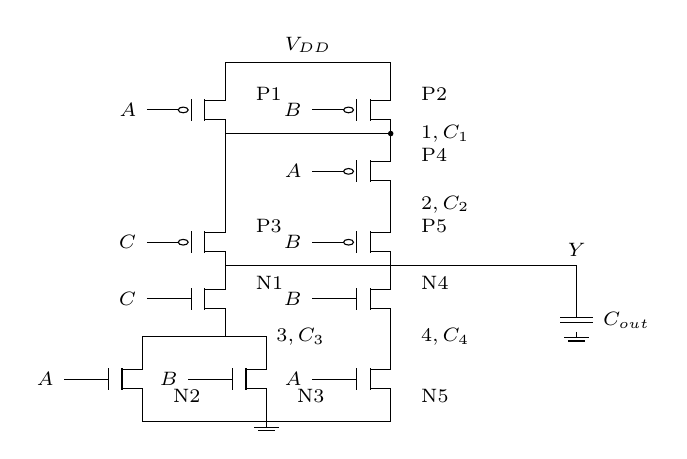
\begin{tikzpicture}[x=1.05cm,y=.6cm,font=\scriptsize]
\mos{1}{6}{A}{1}\mos{3}{6}{B}{1}\draw(1.25,6.5)--(1.25,7)--(3.25,7)--(3.25,6.5);\node[above]at(2.25,7){$V_{DD}$};\node[right]at(1.5,6.35){P1};\node[right]at(3.5,6.35){P2};
\draw(1.25,5.5)--(3.25,5.5);\fill(3.25,5.5)circle(1pt);\node[right]at(3.5,5.5){$1,C_1$};
\mos{3}{4.7}{A}{1}\draw(3.25,5.5)--(3.25,5.2);\node[right]at(3.5,5.05){P4};\draw(3.25,4.2)--(3.25,4);\node[right]at(3.5,4){$2,C_2$};
\mos{1}{3.2}{C}{1}\mos{3}{3.2}{B}{1}\draw(1.25,5.5)--(1.25,3.7);\draw(3.25,4)--(3.25,3.7);\node[right]at(1.5,3.5500000000000003){P3};\node[right]at(3.5,3.5500000000000003){P5};
\draw(1.25,2.7)--(3.25,2.7)--(5.5,2.7)node[above]{$Y$};\draw(5.5,2.7)--(5.5,1.6);\draw(5.3,1.6)--(5.7,1.6) (5.3,1.5)--(5.7,1.5);\grd{5.5}{1.3}\node[right]at(5.7,1.55){$C_{out}$};
\mos{1}{2}{C}{0}\mos{3}{2}{B}{0}\draw(1.25,2.7)--(1.25,2.5);\draw(3.25,2.7)--(3.25,2.5);\node[right]at(1.5,2.35){N1};\node[right]at(3.5,2.35){N4};
\draw(1.25,1.5)--(1.25,1.2)--(.25,1.2)--(.25,.8);\draw(1.25,1.2)--(1.75,1.2)--(1.75,.8);\node[right]at(1.75,1.2){$3,C_3$};\draw(3.25,1.5)--(3.25,.8);\node[right]at(3.5,1.2){$4,C_4$};
\mos{0}{.3}{A}{0}\mos{1.5}{.3}{B}{0}\mos{3}{.3}{A}{0}\node[right]at(.5,-0.04999999999999999){N2};\node[right]at(2,-0.04999999999999999){N3};\node[right]at(3.5,-0.04999999999999999){N5};
\draw(.25,-.2)--(.25,-.6)--(3.25,-.6)--(3.25,-.2);\draw(1.75,-.2)--(1.75,-.6);\grd{1.75}{-.6}
\end{tikzpicture}\end{center}
The PDN implements $H=C(A+B)+AB=AB+AC+BC$. Thus
\[\boxed{Y=\overline{AB+C(A+B)}}.\]
Its gate-level realization is an AND for AB and an AND for $C(A+B)$, followed by NOR. This preserves the final complement, which is missing in the photographed handwritten formula.
\begin{center}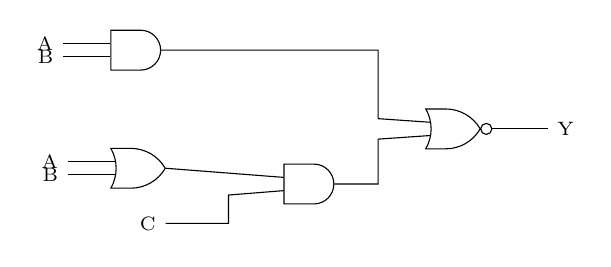
\begin{tikzpicture}[font=\scriptsize]
\node[and gate US,draw,logic gate inputs=nn](p)at(1,1){};\node[or gate US,draw,logic gate inputs=nn](s)at(1,-.5){};\node[and gate US,draw,logic gate inputs=nn](q)at(3.2,-.7){};\node[nor gate US,draw,logic gate inputs=nn](y)at(5,0){};
\foreach\g in{p,s}{\draw(\g.input 1)--++(-.6,0)node[left]{A};\draw(\g.input 2)--++(-.6,0)node[left]{B};}\draw(s.output)--(q.input 1);\draw(q.input 2)--(2.2,-.84)--(2.2,-1.2)--(1.4,-1.2)node[left]{C};\draw(p.output)--(4.1,1)--(4.1,.13)--(y.input 1);\draw(q.output)--(4.1,-.7)--(4.1,-.13)--(y.input 2);\draw(y.output)--++(.7,0)node[right]{Y};
\end{tikzpicture}\end{center}
For (b), state the simple RC convention: the Elmore first moment of each final ON network, with connected capacitances fully unsettled. It estimates transition time without a common log/10--90\% factor; exact waveforms and internal initial voltages are not supplied. Let $p_i=R_{Pi}$, $n_i=R_{Ni}$, and $c=C_{out}$, $p_{12}=p_1\parallel p_2$.

\textbf{Rise:} common input controls must be respected. The three potentially worst final high states give
\begin{align*}
t_r(001)&=p_{12}(C_1+C_2+c+C_3)+p_4(C_2+c+C_3)+p_5(c+C_3),\\
t_r(010)&=p_1(C_1+C_2+c+C_4)+p_3(c+C_4),\\
t_r(100)&=p_2(C_1+C_2+c)+p_3(C_2+c),\\
\boxed{t_{r,worst}}&=\boxed{\max\{t_r(001),t_r(010),t_r(100)\}}.
\end{align*}
In 001, N1 connects dangling $C_3$ to Y. In 010, P4 connects dangling $C_2$ to node 1 and N4 connects dangling $C_4$ to Y. In 100, P5 connects $C_2$ to Y. A=0,B=0 is required for P4/P5 to conduct together, so P1 and P2 then conduct \emph{in parallel}; choosing only the slower of those two in that series path is not a reachable state. At 000, P3 adds a parallel route and the nMOS dangling loads disappear, so its first moment cannot exceed the 001 expression with positive R/C.

\textbf{Fall:} the corresponding three potentially worst low states give
\begin{align*}
t_f(011)&=(n_1+n_3)(c+C_4)+n_3C_3,\\
t_f(101)&=(n_1+n_2)(c+C_2)+n_2C_3,\\
t_f(110)&=(n_4+n_5)(c+C_1)+n_5C_4,\\
\boxed{t_{f,worst}}&=\boxed{\max\{t_f(011),t_f(101),t_f(110)\}}.
\end{align*}
In 101, P5 attaches $C_2$ to Y; in 110, P3 attaches $C_1$ to Y. In 011, N4 attaches floating $C_4$ to Y. At 111, both ground branches conduct and remove that floating case; its moment is bounded by 011. Thus a resistor-path sum multiplied only by $C_{out}$ misses specified node capacitances and can misidentify the worst case.

These are network first-moment estimates, not an assertion that every capacitor can begin at zero/full supply in every real predecessor state. If ``simple RC'' means excluding all dangling opposite-network capacitors, remove the explicitly identified $C_3/C_4/C_2/C_1$ additions; that is an extra approximation, not the literal full conducting graph. The saved verifier exhausts all eight switch states and checks the formulas against nodal linear equations for varied positive R/C values.
\textbf{Verification.} Complete MOS graphs, 16 Q1 words, 32 Q4 words, all eight Q6 words, ordered charging events and RC moments are saved. The reconstructed figures are editable and retain the printed connections. Student annotations are corrected after original-first derivation.\end{document}